\documentclass[a4paper]{article}

\usepackage[T1]{fontenc}
\usepackage[utf8]{inputenc}
\usepackage[italian]{babel}
\usepackage[a4paper]{geometry}
\usepackage[hidelinks]{hyperref}
\usepackage{eurosym}
\usepackage{caption, subcaption}
\usepackage{tikz, circuitikz}
\usepackage{pgf-umlcd, pgf-umlsd}

\renewcommand{\umltextcolor}{black}
\renewcommand{\umldrawcolor}{black}
\renewcommand{\umlfillcolor}{white}

\setlength{\parskip}{1.2ex}
\setlength{\parindent}{0em}
\clubpenalty = 100
\widowpenalty = 100

\title{CHIP-8 STM32}
\date{\today}
\author{Federico Bruzzone, Lorenzo Ferrante, Andrea Longoni \\
\footnotesize \texttt{\{federico.bruzzone, lorenzo.ferrante1, andrea.longoni3\}@studenti.unimi.it} \\ }

\begin{document}
\maketitle

\section{Introduzione}

% TODO: includere una foto dell'emulatore finito e funzionante

CHIP-8 è un linguaggio di programmazione creato a metà degli anni '70
da Joseph Weisbecker per semplificare lo sviluppo di videogiochi per
microcomputer a 8 bit. I programmi CHIP-8 vengono interpretati da una
macchina virtuale che è stata estesa parecchie volte nel corso degli
anni, tra le versioni più adottate citiamo S-CHIP e la più recente
XO-CHIP.

La semplicità dell'interprete in aggiunta alla sua lunga storia e
popolarità hanno fatto sì che emulatori e programmi CHIP-8 vengano
realizzati ancora oggi.
Nel corso degli anni molti videogiochi storici sono stati riscritti
in CHIP-8 tra cui Pong, Space Invaders e Tetris.

Lo scopo del progetto è quello di costruire un emulatore CHIP-8 e
S-CHIP in grado di funzionare su un microcontrollore STM32.

In questo documento ci riferiremo alla macchina virtuale che
interpreta programmi CHIP-8 con "interprete". Mentre utilizzeremo
"emulatore" per indicare l'interprete assieme ad una sua
implementazione (o "port"), ovvero un programma che gestisce
l'audio, il video, l'input da tastiera e interagisce con l'API della
macchina virtuale.

% TODO: migliorare lo scopo del progetto e accennare alle periferiche

\section{Hardware}

% TODO

\subsection{Schema di collegamento}

% TODO

\begin{figure}
\begin{center}
    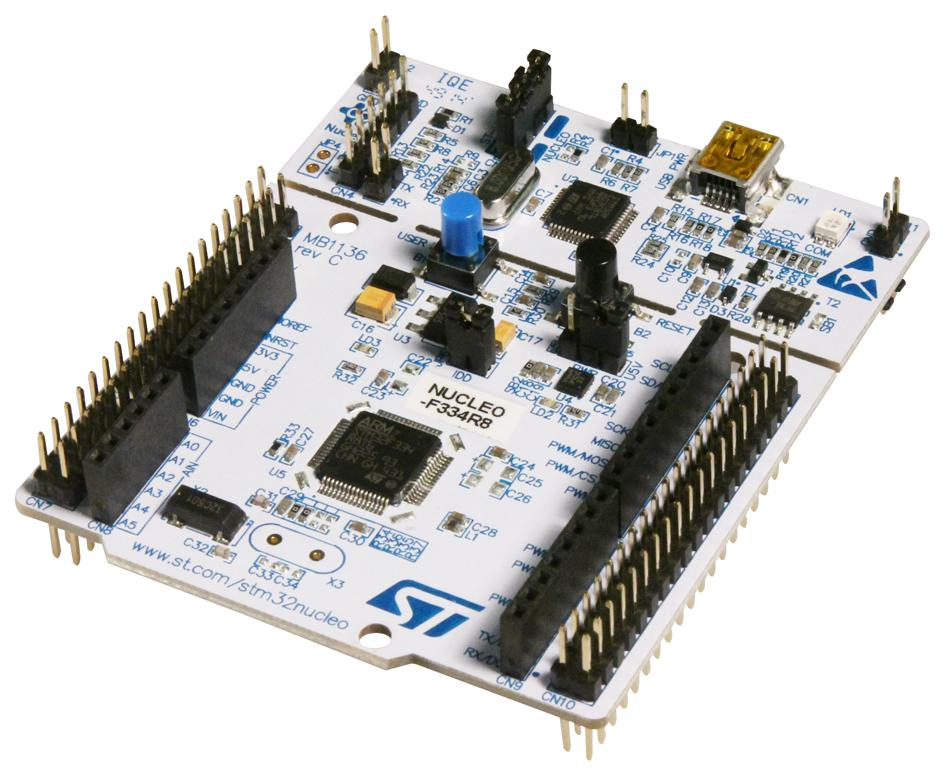
\includegraphics[scale=0.20]{figures/stm32f334.jpg}
\end{center}
\caption{Il microcontrollore \texttt{STM32F334R8T6}.}
\label{fig:stm32f334}
\end{figure}

\begin{figure}[h]
    \begin{subfigure}[b]{0.45\textwidth}
        \begin{center}
            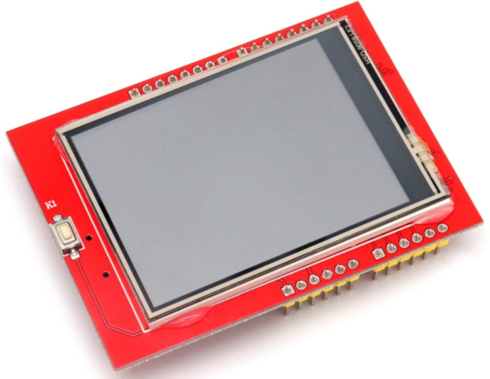
\includegraphics[scale=0.4]{figures/ili9341.png}
        \end{center}
        \caption{Lo schermo ILI9341.}
        \label{fig:ili9341}
    \end{subfigure}
    \hfill
    \begin{subfigure}[b]{0.45\textwidth}
        \begin{center}
            \begin{tikzpicture}[x=0.015cm, y=0.015cm, scale=0.75, transform shape]
                \draw   (120, 90) -- (320,90) -- (320,480) -- (120,480) -- cycle ;

\draw  [fill={rgb, 255:red, 255; green, 255; blue, 255 }  ,fill opacity=1 ]  (90,100)  --  (200,100) -- (200,130) --  (90,130) -- cycle;
\draw  [fill={rgb, 255:red, 255; green, 255; blue, 255 }  ,fill opacity=1 ]  (90,130)  --  (200,130) -- (200,160) --  (90,160) -- cycle;
\draw  [fill={rgb, 255:red, 255; green, 255; blue, 255 }  ,fill opacity=1 ]  (90,160)  --  (200,160) -- (200,190) --  (90,190) -- cycle;
\draw  [fill={rgb, 255:red, 255; green, 255; blue, 255 }  ,fill opacity=1 ]  (90,190)  --  (200,190) -- (200,220) --  (90,220) -- cycle;
\draw  [fill={rgb, 255:red, 255; green, 255; blue, 255 }  ,fill opacity=1 ]  (90,220)  --  (200,220) -- (200,250) --  (90,250) -- cycle;
\draw  [fill={rgb, 255:red, 255; green, 255; blue, 255 }  ,fill opacity=1 ]  (90,250)  --  (200,250) -- (200,280) --  (90,280) -- cycle;
\draw  [fill={rgb, 255:red, 255; green, 255; blue, 255 }  ,fill opacity=1 ]  (90,280)  --  (200,280) -- (200,310) --  (90,310) -- cycle;
\draw  [fill={rgb, 255:red, 255; green, 255; blue, 255 }  ,fill opacity=1 ]  (90,310)  --  (200,310) -- (200,340) --  (90,340) -- cycle;
\draw  [fill={rgb, 255:red, 255; green, 255; blue, 255 }  ,fill opacity=1 ]  (90,340)  --  (200,340) -- (200,370) --  (90,370) -- cycle;
\draw  [fill={rgb, 255:red, 255; green, 255; blue, 255 }  ,fill opacity=1 ]  (90,370)  --  (200,370) -- (200,400) --  (90,400) -- cycle;
\draw  [fill={rgb, 255:red, 255; green, 255; blue, 255 }  ,fill opacity=1 ]  (90,400)  --  (200,400) -- (200,430) --  (90,430) -- cycle;
\draw  [fill={rgb, 255:red, 255; green, 255; blue, 255 }  ,fill opacity=1 ]  (90,430)  --  (200,430) -- (200,460) --  (90,460) -- cycle;

\draw  [fill={rgb, 255:red, 255; green, 255; blue, 255 }  ,fill opacity=1 ] (250,100)  --  (380,100) -- (380,130) --  (250,130) -- cycle;
\draw  [fill={rgb, 255:red, 255; green, 255; blue, 255 }  ,fill opacity=1 ] (250,130)  --  (380,130) -- (380,160) --  (250,160) -- cycle;
\draw  [fill={rgb, 255:red, 255; green, 255; blue, 255 }  ,fill opacity=1 ] (250,160)  --  (380,160) -- (380,190) --  (250,190) -- cycle;
\draw  [fill={rgb, 255:red, 255; green, 255; blue, 255 }  ,fill opacity=1 ] (250,190)  --  (380,190) -- (380,220) --  (250,220) -- cycle;
\draw  [fill={rgb, 255:red, 255; green, 255; blue, 255 }  ,fill opacity=1 ] (250,220)  --  (380,220) -- (380,250) --  (250,250) -- cycle;
\draw  [fill={rgb, 255:red, 255; green, 255; blue, 255 }  ,fill opacity=1 ] (250,250)  --  (380,250) -- (380,280) --  (250,280) -- cycle;
\draw  [fill={rgb, 255:red, 255; green, 255; blue, 255 }  ,fill opacity=1 ] (250,280)  --  (380,280) -- (380,310) --  (250,310) -- cycle;
\draw  [fill={rgb, 255:red, 255; green, 255; blue, 255 }  ,fill opacity=1 ] (250,310)  --  (380,310) -- (380,340) --  (250,340) -- cycle;
\draw  [fill={rgb, 255:red, 255; green, 255; blue, 255 }  ,fill opacity=1 ] (250,340)  --  (380,340) -- (380,370) --  (250,370) -- cycle;


\draw (90,460) node [anchor=north west][inner sep=0.75pt]   [align=left] {$\displaystyle SD\_SCK$};
\draw (90,430) node [anchor=north west][inner sep=0.75pt]   [align=left] {$\displaystyle SD\_DO$};
\draw (90,400) node [anchor=north west][inner sep=0.75pt]   [align=left] {$\displaystyle SD\_DI$};
\draw (90,370) node [anchor=north west][inner sep=0.75pt]   [align=left] {$\displaystyle SD\_SS$};
\draw (90,340) node [anchor=north west][inner sep=0.75pt]   [align=left] {$\displaystyle LCD\_D1$};
\draw (90,310) node [anchor=north west][inner sep=0.75pt]   [align=left] {$\displaystyle LCD\_D0$};
\draw (90,280) node [anchor=north west][inner sep=0.75pt]   [align=left] {$\displaystyle LCD\_D7$};
\draw (90,250) node [anchor=north west][inner sep=0.75pt]   [align=left] {$\displaystyle LCD\_D6$};
\draw (90,220) node [anchor=north west][inner sep=0.75pt]   [align=left] {$\displaystyle LCD\_D4$};
\draw (90,190) node [anchor=north west][inner sep=0.75pt]   [align=left] {$\displaystyle LCD\_D5$};
\draw (90,160) node [anchor=north west][inner sep=0.75pt]   [align=left] {$\displaystyle LCD\_D3$};
\draw (90,130) node [anchor=north west][inner sep=0.75pt]   [align=left] {$\displaystyle LCD\_D2$};

\draw (250,370) node [anchor=north west][inner sep=0.75pt]   [align=left] {$\displaystyle 3.3V$};
\draw (250,340) node [anchor=north west][inner sep=0.75pt]   [align=left] {$\displaystyle 5V$};
\draw (250,310) node [anchor=north west][inner sep=0.75pt]   [align=left] {$\displaystyle GND$};
\draw (250,280) node [anchor=north west][inner sep=0.75pt]   [align=left] {$\displaystyle LCD\_RD$};
\draw (250,250) node [anchor=north west][inner sep=0.75pt]   [align=left] {$\displaystyle LCD\_WR$};
\draw (250,220) node [anchor=north west][inner sep=0.75pt]   [align=left] {$\displaystyle LCD\_RS$};
\draw (250,190) node [anchor=north west][inner sep=0.75pt]   [align=left] {$\displaystyle LCD\_CS$};
\draw (250,160) node [anchor=north west][inner sep=0.75pt]   [align=left] {$\displaystyle LCD\_RST$};
\draw (250,130) node [anchor=north west][inner sep=0.75pt]   [align=left] {$\displaystyle F\_CS$};

            \end{tikzpicture}
        \end{center}
        \caption{Pinout dello schermo \texttt{ILI9341}.}
        \label{fig:pinout_ili}
    \end{subfigure}
\end{figure}

\subsection{Materiali e costi} % ALT: Componenti e costi / Componenti utilizzati e relativi costi

\begin{center}
    \begin{table}[ht]
        \centering
        \begin{tabular}{|llll|l|}
            \hline
            \multicolumn{1}{|l|}{\textbf{Descrizione}}          & \multicolumn{1}{l|}{\textbf{Modello}}       & \multicolumn{1}{l|}{\textbf{Costo unitario}} & \textbf{Unità} & \textbf{Costo} \\ \hline
            \multicolumn{1}{|l|}{Microcontrollore}       & \multicolumn{1}{l|}{STM32 F334R8T6}         & \multicolumn{1}{l|}{14.99}                   & 1               & 14.99          \\ \hline
            \multicolumn{1}{|l|}{Schermo}                & \multicolumn{1}{l|}{ILI9341 2.4"}           & \multicolumn{1}{l|}{6.50}                    & 1               & 6.50           \\ \hline
            \multicolumn{1}{|l|}{Tastierino}          & \multicolumn{1}{l|}{Matrix keypad 4$\times$4} & \multicolumn{1}{l|}{3.99}                    & 1               & 3.99           \\ \hline
            \multicolumn{1}{|l|}{Beeper}                 & \multicolumn{1}{l|}{}                       & \multicolumn{1}{l|}{0.99}                    & 1               & 0.99           \\ \hline
            \multicolumn{1}{|l|}{Breadboard e cablaggio} & \multicolumn{1}{l|}{}                       & \multicolumn{1}{l|}{4.99}                    & 1               & 4.99           \\ \hline
            \multicolumn{4}{|r|}{\textbf{Totale}}                                                      & 31.50\euro    \\ \hline
        \end{tabular}
        \caption{
            Materiali utilizzati per la costruzione del progetto. I costi indicati provengono da negozi online come Amazon e eBay.
        }
    \end{table}
\end{center}

\section{Software}

Il nostro software si divide in due componenti principali:
l'interprete CHIP-8 e l'infrastruttura necessaria per "portarlo"
su un microcontrollore STM32, ovvero l'interfaccia con lo schermo
e i gestori per la scheda microSD, per il keypad e per il beeper.

\subsection{Interprete CHIP-8}

Abbiamo deciso di scrivere l'interprete da zero e per farlo è
stato necessario consultare le specifiche (de facto standard)
che definiscono il comportamento di un interprete
CHIP-8 \cite{cowgod:chip8} e S-CHIP \cite{cowgod:schip}.

L'interprete ha un'architettura basata su registri e possiede 4 KB
di memoria, 16 registri general purpose, un registro per gli
indirizzi di memoria, un registro per il delay timer,
un registro per il sound timer, uno stack per gestire le
chiamate a subroutine, uno stack pointer e un program counter.

Il delay timer viene utilizzato come cronometro mentre il sound
timer è utilizzato per gestire gli effetti sonori, quando il suo
valore è diverso da zero, l'emulatore attiva il beeper.

% Ad ogni ciclo di esecuzione l'interprete effettua il fetch
% dell'istruzione puntata dal program counter in memoria,
% la decodifica e la esegue.

Sono supportate 45 istruzioni diverse, ciascuna delle
quali è rappresentata da uno specifico opcode in cui al suo interno
sono passati anche eventuali parametri.

Il programma è scritto in C99, non ha I/O ed è freestanding
\cite{n1256:conformance}, ovvero non dipende dalla libreria
standard del C. Tutto questo è mirato a rendere l'interprete
altamente portabile.

Per rimuovere la dipendenza dalla libreria standard del C è stato
necessario includere alcune funzioni direttamente da libgcc, trovare
un modo alternativo per implementare le asserzioni e includere una
funzione ad hoc per la generazione di numeri casuali.

Infine per testare più comodamente l'interprete abbiamo sviluppato
un semplice emulatore su desktop utilizzando SDL2
\cite{libsdl:about}, una libreria scritta in C che consente di
gestire audio, video e input da tastiera.
In seguito l'interprete è stato sottoposto ad un'apposita
test suite \cite{github:chip8-test-suite} che mira a verificare
il comportamento corretto di ciascun opcode.

\subsubsection{Gestione del timing}

Uno dei problemi principali durante lo sviluppo di un emulatore è
la gestione del timing, in particolare è necessario limitare la
"velocità" dell'emulatore bloccando temporaneamente la sua
esecuzione.

Inoltre abbiamo dovuto disaccoppiare la frequenza dell'interprete
(regolabile dal giocatore) dalla frequenza del delay timer e del
sound timer (costante a 60 Hz). Dove con frequenza dell'interprete
ci riferiamo al numero di istruzioni che esegue ogni frame.

% Durante lo sviluppo abbiamo testato due soluzioni diverse.

Inizialmente abbiamo optato per la gestione di una singola istruzione
per ciclo di esecuzione, di conseguenza il ritardo del game loop
risultava variabile e dipendeva dalla frequenza selezionata dal
giocatore. Per assicurare una frequenza di 60 Hz i timer
venivano decrementati ogni n-esima iterazione del game loop, dove
n = FREQ / 60. Ad esempio se FREQ = 540, i timer venivano
decrementati ogni 9º ciclo.

Purtroppo però questo approccio presenta un problema non
trascurabile, ovvero effettua una chiamata ad una funzione
simil-sleep per un periodo molto breve dopo ogni istruzione.
Ad esempio se FREQ = 540, il ritardo di una sleep sarebbe solo
di 1.85 ms, e questo genere di funzione non offre una precisione
simile. Per questo motivo abbiamo optato per una soluzione
differente.

Abbiamo fissato il ritardo del game loop a 16.666 ms, un valore
sufficientemente alto da non avere problemi di granularità. Inoltre
in questo modo otteniamo un frame rate di 60 fps esatti. Avendo
reso il ritardo costante abbiamo dovuto rendere variabile il numero
di istruzioni gestite durante un ciclo di esecuzione. In particolare
vengono gestite n istruzioni per ciclo, dove n = FREQ / 60.
Ad esempio se FREQ = 540, vengono gestite 9 istruzioni per ciclo.
A questo punto dato che il game loop viene ripetuto con una
frequenza di 60 Hz risulta banale gestire la frequenza dei timer.

Sono state considerate anche eventuali problematiche che sarebbero
potute sorgere con questo approccio. In particolare non tutte le
istruzioni impiegano lo stesso tempo per essere eseguite, ma
fortunatamente anche l'istruzione più lenta richiede una quantità
trascurabile di tempo. Ciò significa che possiamo
comportarci come se tutte le istruzioni richiedessero il medesimo
tempo.

\subsubsection{Ottimizzazioni}

\begin{figure}
    \begin{center}
        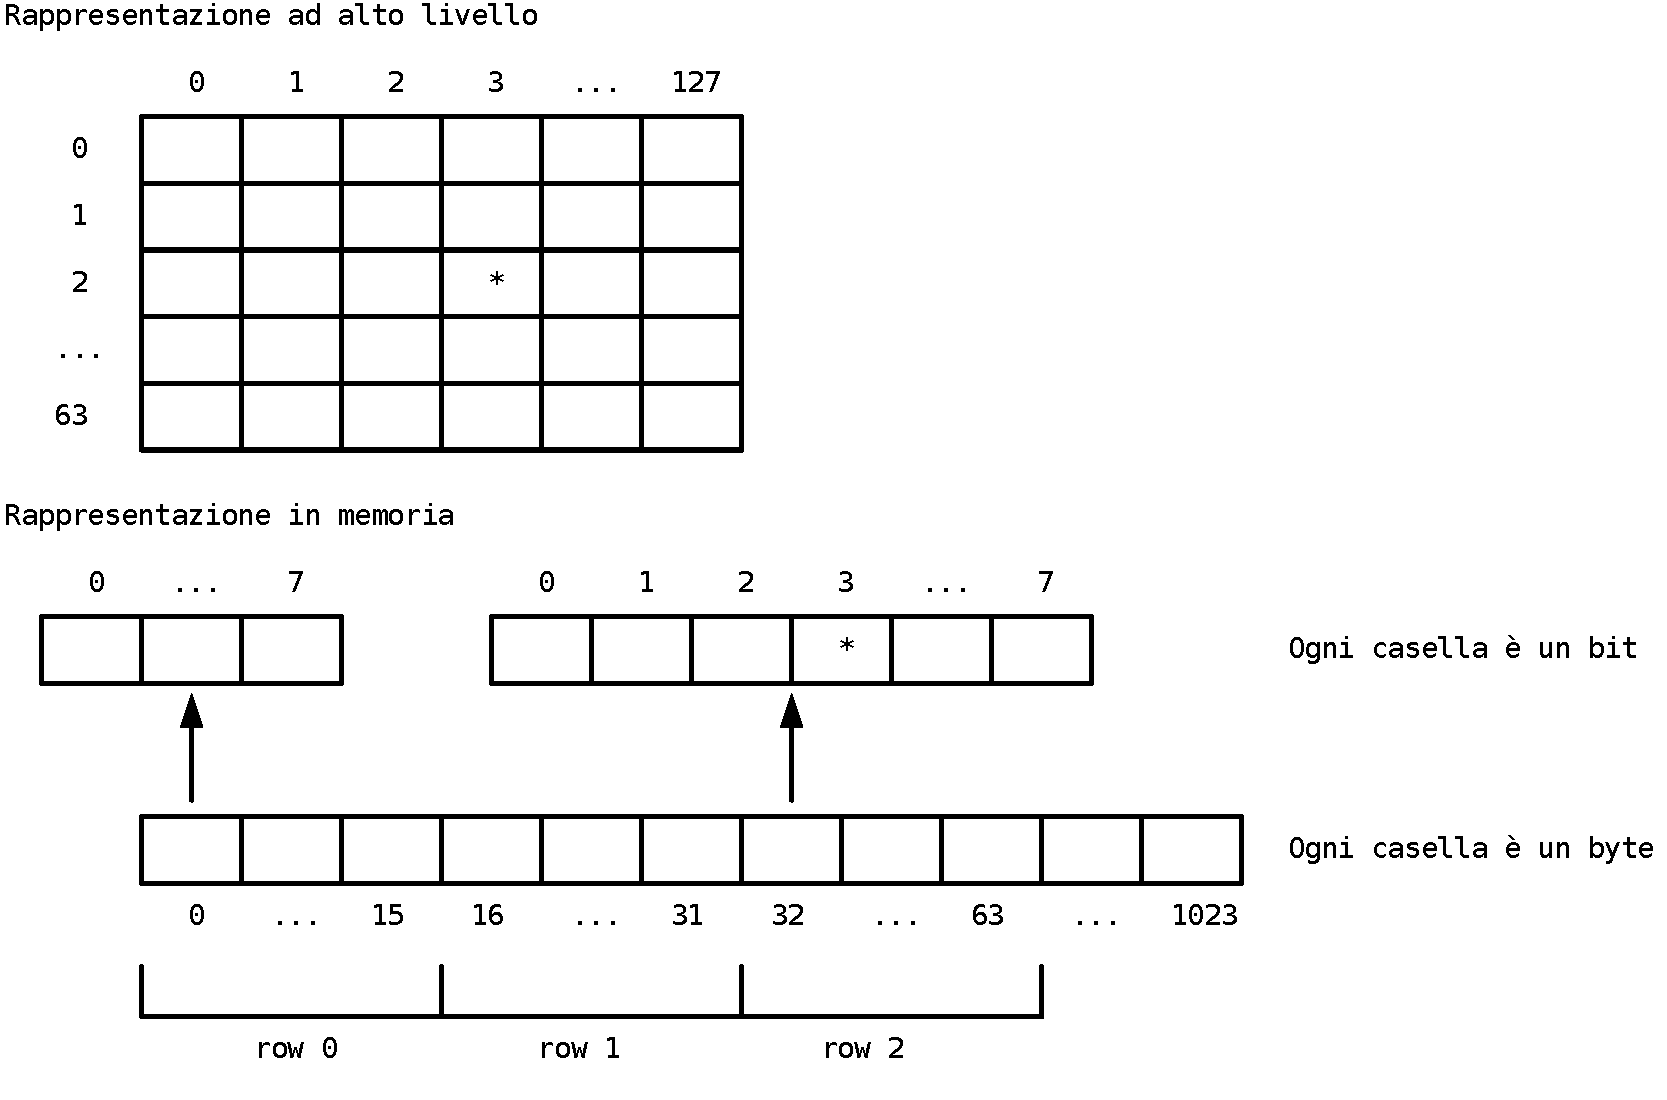
\includegraphics[scale=0.50]{figures/screenopt.pdf}
    \end{center}
    \caption{Esempio della mappatura di un pixel.}
    \label{fig:screenopt}
\end{figure}

È stato necessario introdurre delle ottimizzazioni all'interno
dell'interprete per poterlo far girare su un microcontrollore.

L'ottimizzazione principale è legata alla rappresentazione dello
schermo in memoria. Ad alto livello lo schermo può essere visto
come una matrice di 128x64 pixel monocromi. Una rappresentazione
simile occuperebbe 8192 byte, dato che ciascun pixel verrebbe
rappresentato da un byte.

Purtroppo il nostro microcontrollore ha a disposizione solamente
16 KB di SRAM, di conseguenza una soluzione simile non è praticabile.

Per questo motivo abbiamo deciso di rappresentare lo schermo come
un array unidimensionale di 1024 byte, dove ciascun pixel viene
rappresentato da un singolo bit. In questo modo otteniamo un
risparmio di spazio pari a ben l'87.5\%.

Questa decisione ha aggiunto però un livello di indirezione dato
che una coordinata ad alto livello sulla matrice 128x64 deve essere
mappata ad una coordinata "in memoria".

Un'ulteriore ottimizzazione viene resa disponibile attraverso l'API
dell'interprete sotto forma di una funzione che consente al chiamante
di controllare se l'array che rappresenta lo schermo è stato
modificato nell'ultimo ciclo di esecuzione. In questo modo la grafica
viene renderizzata dal chiamante solo quando è effettivamente
necessario.

\subsubsection{Comportamenti ambigui}

Gli interpreti CHIP-8 e S-CHIP hanno sviluppato molteplici
comportamenti ambigui nel corso degli anni. Questi cosiddetti
"quirk" variano in base alle piattaforme per cui è stato sviluppato
l'interprete. Ad esempio gli interpreti per calcolatrici HP48
presentano un comportamento leggermente diverso durante l'esecuzione
delle istruzioni di SHIFT.

Questi comportamenti ambigui si propagano fino ai programmatori
CHIP-8 che si appoggiano a quest'ultimi e scrivono videogiochi che
non sono del tutto compatibili con interpreti più vecchi. Per evitare
questa frammentazione è necessario supportare le piattaforme
principali e i loro quirk.

Il nostro interprete supporta CHIP-8, CHIP-48, S-CHIP 1.0 e
S-CHIP 1.1, in questo modo è in grado di eseguire la stragrande
maggioranza dei videogiochi reperibili in rete.

\subsection{Porting su STM32}

\subsubsection{Interfaccia con lo schermo}

\subsubsection{Gestori per le ulteriori periferiche}

\subsubsection{Menù di selezione}

\subsection{Architettura}

% TODO: aggiornare il class diagram e il sequence diagram

% \section{Assemblaggio}

% TODO

\section{Analisi del consumo energetico} % ALT: Alimentazione e consumi

% TODO

\section{Considerazioni finali} % ALT: Conclusioni e sviluppi futuri

% TODO

\addcontentsline{toc}{section}{Riferimenti bibliografici}
\bibliographystyle{plain}
\bibliography{report}

\end{document}
